% related work = related scientific articles
% NOT engineering (tsap, at3, tribler-mobile (ppsp-twitter))
% https://scholar.google.nl/scholar?hl=en&q=video+on+demand+android&btnG=&as_sdt=1%2C5&as_sdtp=


\chapter{Introduction}
% 3 to 4 pages with screenshots
% related work in citations in between text

In the era of social media people on earth are more connected then ever before.
%stats

However not every place on earth has an uncensored Internet connection, or has one that can be shut down with the push of a button.
%examples

Although smart phones have brought the Internet into the hands of people, this mobile device is not capable of overturning the power of the Internet-kill-switch, yet.
This is about to change as the self-organising video-on-demand platform Tribler is going to make the jump to mobile devices.
% relevance
A big part of social media is video sharing and streaming.
%stats
There is a great interest in this considering the amount of websites and apps available for streaming video-on-demand services.
%list apps?
Huge video streaming providers like Youtube, Twitch, Periscope, etc. currently dominate the market.
%stats
The problem with those is that none of them are server-less and do not  provide anonymity in any shape or form.
%why

%first point
With servers central to their design they create a single point of failure, even in a decentralized set-up.
Several natural disasters have taken out the necessary infrastructure on numerous occasions for a prolonged period of time.
%examples
Especially in situations like these, people need to communicate and coordinate their efforts to restore safety.
Social media has played a major role in recent calamities when people could mark themselves as safe, effectively broadcasting that information to all their family and friends on social media, instead of contacting them one by one or not at all due to congestion in the communication channels.
So the advantages are obvious, and the vulnerability of central elements underlying current social media too.

%second point
The lack of anonymity becomes a problem when the users privacy is being invaded.
Revealing personal information can be deduced from search queries for example, or associations on social platforms.
When this information can be used for targeted advertising it becomes very valuable, and creates an incentive for the parties that have access to this information to sell it to third parties.
In fact the business model of social media appears to be serving targeted advertisements to its users on behalf of third parties.
What's even worse is social media integrated into regular websites to de-anonymize and track the whereabouts of users even outside of the social media realm.
Whenever users lose control over their privacy it becomes a serious problem.

Various initiatives have been started to deal with one or both of these problems.
Figure \ref{fig:youbroketheinternet} shows a mapping of projects that are or have been working on that.
%From re-decentralized: top projects that match/compare.
\\
\begin{figure}[h]
	\centering
	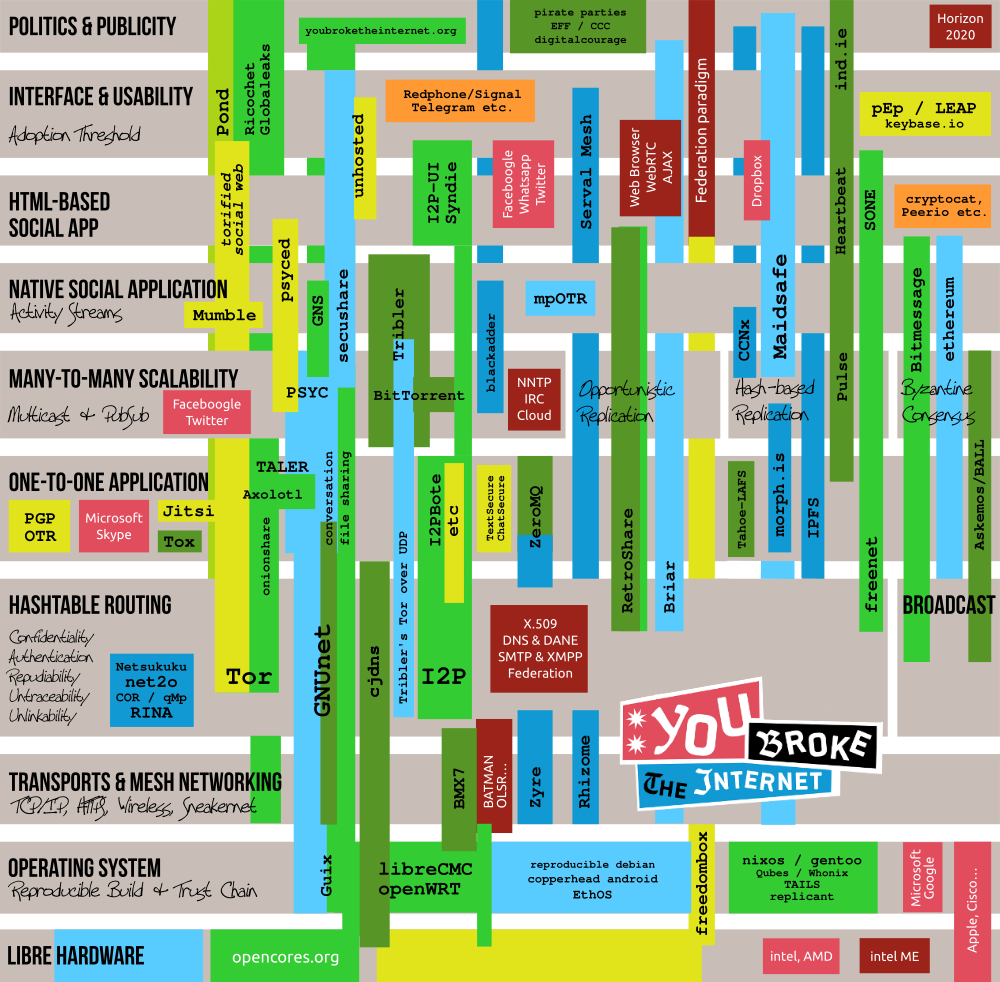
\includegraphics[width=\textwidth]{youbroketheinternet}
	\caption{Map of projects trying to fix the Internet according to youbroketheinternet.org, last updated October 2015\\
		\\
		Colour coding:\\
		\\
		\textcolor[RGB]{51,204,51}{Green:} Projects that are available today.\\
		\textcolor[RGB]{86,149,38}{Dark green:} Projects that are available, but are not fully protective of meta-data.\\
		\textcolor[RGB]{89,204,255}{Blue:} Projects in development.\\
		\textcolor[RGB]{17,153,211}{Dark blue:} Projects in development which will have little or no protection of meta-data (but that does not mean they can't be an excellent piece in the general puzzle).\\
		\textcolor[RGB]{226,228,27}{Yellow:} Projects that may be okay but depend too much on the security of servers.\\
		\textcolor[RGB]{255,153,51}{Orange:} Products whose end-to-end encrypting client side has been open-sourced but whose server side remains proprietary.\\
		\textcolor[RGB]{225,77,93}{Red:} Brands that currently occupy the respective layers with unsafe technology.\\
		\textcolor[RGB]{155,35,25}{Dark red:} Possibly cool but unsafe technologies that we need to replace.}
	\label{fig:youbroketheinternet}
\end{figure}

% Youtube screenshot, GNUnet



being first
engineering perfection
time to market
popularity
make a difference
Tribler mobile vs periscope
fully functional prototype, but poor user interface (unpolished)
real world impact proven insufficient
we want to change the world implicit


\section{Tribler}
% tribler and dispersy intro, what is it (read thesis independently)

Tribler introduces a server-less video-sharing platform with privacy enhancing technologies and giving a Youtube-like, social media experience at the same time.
The capability of hiding your identity is greatly advantageous to the user if his or her human rights are violated, like free speech.

The server-less technique of Tribler is resistant to Internet kill-switches that are typically deployed for the purpose of censorship.


